% durch Austauschen dieser Zeilen kann die Sprache des Templates geändert werden
\PassOptionsToPackage{main=ngerman}{babel}
%\PassOptionsToPackage{main=english}{babel}

\documentclass[thesis]{mi-document}

% Microtypografie aktivieren
\usepackage{microtype}

\bachelor % im Falle einer Masterarbeit \master

% Variablen, die für das Deckblatt und Metadaten verwendet werden
\title{Evaluierung von Einsatzmöglichkeiten einer Deep Learning Applikation zur Detektion gelabelter Merkmale in Bildern}
\author{Amina Kasa}
\semester{Sommersemester 2024}
\course{Bachelorarbeit}
\module{Fakultät Informatik und Mathematik}
\dozent{Prof. Dr. Timo Baumann}
\studid{3190755}
\studSemester{Medizinische Informatik}
\phone{0941/133742666} % Optional
\studSubject{Medizinische Informatik}
\firstReviewer{Prof. Dr. Timo Baumann}
\secondReviewer{Prof. Dr. Brijnesh Jain}
\advisor{GEFASOFT Automatisierung und Software GmbH}
\address{Klenzestr. 2a, 93051 Regensburg}{} % Optional
\mail{kasaamina@gmail.com}
\studMail{amina.kasa@st.oth-regensburg.de}
\dateHandedIn{05.02.2025}
\keywords{Enter;key;words;here}

\bibliographystyle{apacite}

% Falls Sie die Abkürzung zum Einbinden von Grafiken benutzen möchten. Erläuterung fnden Sie im Abschnitt zu Abbildungen.
\newcommand*{\image}[2]{
	\begin{figure}
	\centering
	\includegraphics[width=0.5\textwidth]{{images/#1}}
	\caption{#2}
	\label{fig:#1}
	\end{figure}
}

\usepackage{emptypage}
\pagenumbering{roman}

\usepackage[acronym]{glossaries}
\makeglossaries


\begin{document}
% ---------------------------------------------------------------

 % Die Nummerierung beginnt mit der Titelseite (= Seite 1), soll aber erst ab der ersten Inhaltsseite (Einleitung) angezeigt werden.
    \pagestyle{empty}


% Das Deckblatt erstellen
    \maketitle
 % ---------------------------------------------------------------
 
%\begin{singlespace}
\pagestyle{plain}
\KOMAoptions{parskip=full}
% Erklärung zur Urherberschaft (urheberschaft.tex) anhängen
\addchap*{}
\centering
\LARGE
\textbf{Erklärung zur Bachelorarbeit von}\\

\RaggedRight
\vspace{60pt}

\normalsize
\doublespacing
\begin{tabularx}{\linewidth}{@{}l<{:}>{\RaggedRight\arraybackslash}X@{}}
Name&Kasa\\
Vorname&Amina\\
Studiengang&\getStudSubject\\
\end{tabularx}

\vspace{40pt}

\begin{enumerate}
    \item{Mir ist bekannt, dass dieses Exemplar der Bachelorarbeit als Prüfungsleistung in das 
Eigentum der Ostbayrischen Technischen Hochschule Regensburg übergeht.}
    \item{ Ich erkläre hiermit, dass ich diese Bachelorarbeit selbständig verfasst, noch nicht 
anderweitig für Prüfungszwecke vorgelegt, keine anderen als die angegebenen Quellen 
und Hilfsmittel benutzt sowie wörtliche und sinngemäße Zitate als solche gekennzeichnet 
habe.}
\end{enumerate}


\signature

\newpage
 
% Abstract hinzufügen
    \clearpage
    \doublespacing

    \begin{abstract}[ngerman]
Bachelor- und Masterarbeiten beginnen mit einer Zusammenfassung in einer deutschen und englischen Version.
Die Zusammenfassung gibt einen Überblick über Thema und Resultate der Arbeit.
Inhaltlich werden die Zielsetzung, die Methodik, die einzelnen Arbeitsschritte bzw. Gliederungspunkte und die Ergebnisse der Arbeit widergegeben.

Schlecht: „Schon immer haben Menschen Zusammenfassungen geschrieben [Platitüde, keine Zusammenfassung]. In dieser Arbeit wurde in mehreren Studien untersucht, wie Zusammenfassungen wirken. [Was genau wurde untersucht? Was waren die Ergebnisse?]“

Besser: „In dieser Arbeit wurde untersucht, inwiefern das Lesen von Zusammenfassungen das Lesen des kompletten Dokuments ersetzen kann. Dazu wurden zwei Studien mit jeweils 17 Teilnehmern durchgeführt. In der ersten wurde [...]. Diese Ergebnisse zeigen, dass Bedienungsanleitungen und Bilderbücher weniger gut über Zusammenfassungen erschlossen werden können, als Romane oder Sachbücher.“
\end{abstract}

\begin{abstract}[english]
A summary in English. It should be more or less similar to the German Zusammenfassung. Avoid too verbatim translations („In this work it was examined how the reading of ...“)
\end{abstract}

    \clearpage 
    %\stepcounter{page}
% ---------------------------------------------------------------
%Inhaltsverzeichnisse  
\pagestyle{plain}
\singlespacing
\addcontentsline{toc}{chapter}{Inhaltsverzeichnis}
\tableofcontents % Optional
\newpage
%\stepcounter{page}

\addcontentsline{toc}{chapter}{Abbildungsverzeichnis}
\listoffigures % Optional
\newpage
%\stepcounter{page}

\addcontentsline{toc}{chapter}{Tabellenverzeichnis}
\listoftables % Optional
\newpage
%\stepcounter{page}

\addcontentsline{toc}{chapter}{Quellcodeverzeichnis}
\lstlistoflistings % Optional
\newpage

% Abkürzungsverzeichnis
\clearpage
\addcontentsline{toc}{chapter}{Abkürzungsverzeichnis}
\printglossary[type=\acronymtype, title=Abkürzungsverzeichnis]

% --------------------------------------------------------------
\newacronym{ai}{AI}{Artificial Intelligence}
\newacronym{ibv}{IBV}{industrielle Bildverarbeitung}
\newacronym{dl}{DL}{Deep Learning}
\newacronym{cnn}{CNNs}{Convolutional Neural Networks}
\newacronym{knn}{KNNs}{Künstliche Neuronale Netze}
\newacronym{bv}{BV}{Bildverarbeitung}
\newacronym{bvl}{BV-Labor}{Bildverarbeitungs-Labor}
\newacronym{cv}{CV}{Computer Vision}
\newacronym{oe}{OE}{Objekterkennung}
\newacronym{ml}{ML}{Maschinelles Lernen}

\pagenumbering{arabic}
\pagestyle{headings} % Seitennummern und Kapitelbezeichnungen anzeigen
    
    % hier beginnt der eigentliche Inhalt der Arbeit
    \chapter{Einleitung}\label{sec:Einleitung}
\pagestyle{headings} % Seitennummern und Kapitelbezeichnungen anzeigen

Die \gls{ibv} ist ein essenzieller Bestandteil moderner Fertigungsprozesse und Qualitätskontrollsysteme. Als Teilgebiet des maschinellen Sehens, auch bekannt als \gls{cv}, ermöglicht sie Maschinen und Systemen, visuelle Informationen aus Produktionsprozessen und Produkten zu erfassen und zu analysieren. Dadurch können Aufgaben wie \textbf{Qualitätskontrolle}, \textbf{Inspektion}, \textbf{Positionierung} und \textbf{Vermessung} automatisiert durchgeführt werden, was zur Steigerung der Produktqualität und Effizienz der Prozesse und Kostensenkung beiträgt \citep{cognex_grundlagen_nodate}.

Nach \citep{jahne_digitale_2024} ist unter \gls{cv} ein Computersystem zu verstehen, das die gleiche Aufgabe wie ein biologisches System erfüllt, nämlich aus Bildern zu erkennen, was in der Welt ist und wo es sich befindet. Während Menschen aufgrund evolutionärer Entwicklungen visuelle Informationen intuitiv verarbeiten, haben \gls{cv}-Algorithmen nach wie vor Schwierigkeiten, dieselben Aufgaben zuverlässig zu bewältigen \citep[S.~3]{szeliski_computer_2022}. 

In den letzten Jahren allerdings hat die Komplexität industrieller Problemstellungen stark zugenommen, sodass traditionelle Methoden der Bildverarbeitung oft nicht mehr ausreichen \citep[S.~442]{suse_bildverarbeitung_2014}. \gls{knn} übertreffen mittlerweile bei idealen Bilddaten sogar die menschliche Wahrnehmung \citep{dodge_study_2017}. Durch den Einsatz von \gls{dl}-Methoden können komplexe und variierende Prüfaufgaben wie \textbf{Objektdetektion}, \textbf{Bildklassifikation} und \textbf{Segmentierung} effizient automatisiert werden \citep{kaur_systematic_2024, manakitsa_review_2024}.

Der Einsatz von \gls{dl} führt aber auch zu Veränderungen im Gesamtprozess. Neue Teilprozesse wie das Training von \gls{knn} sind bereits hinreichend wissenschaftlich untersucht. Insbesondere erfordern diese Modelle große Mengen an Trainingsdaten, um zuverlässig zu funktionieren, und sind empfindlich gegenüber Bildrauschen und anderen Störfaktoren \citep{dodge_study_2017}. In industriellen Anwendungen stehen jedoch oft nur begrenzte Datenmengen zur Verfügung, und die Bilddaten können aufgrund von Produktionsbedingungen Rauschen oder Qualitätsmängel aufweisen.

\textbf{Ziel dieser Arbeit} ist es daher, die Entwicklung und Evaluierung einer \gls{dl}-Anwendung vorzustellen, die spezifische Merkmale in industriellen Bildern automatisch erkennen und segmentieren kann. Insbesondere wird die UNet-Architektur betrachtet, die sich in ähnlichen Anwendungsfällen bewährt hat.

\section{Hintergrund und Motivation }\label{motivation}

Im Rahmen meines Praxissemesters bei der Gefasoft GmbH in Regensburg hatte ich die Gelegenheit, mich intensiv mit unterschiedlichen Projekten der \gls{ibv} zu befassen. Im Bildverarbeitungs-Labor konnte ich einen tiefen Einblick in die vielfältigen Projekte der Sichtprüfung gewinnen. Zu den typischen Aufgaben in diesem Bereich zählen unter anderem die Objekterkennung, Oberflächeninspektion und Vollständigkeitsprüfung \cite[S. 5]{demant_industrielle_2011}.

Die Umsetzung der genannten Prozesse umfasst eine Reihe von Schritten, die von der Bildaufnahme und -vorverarbeitung bis zur Analyse und Bewertung der Bilddaten reichen (s. Abbildung \ref{fig:vorgehensmodell}). Im Rahmen dessen werden spezifische Vorgaben und Ziele definiert, um die gewünschten Informationen aus einem Bild zu extrahieren und in der realen Welt existierende Objekte zu erfassen. Im Anschluss erfolgt die Separierung der Objekte vom Hintergrund. Diesbezüglich werden Regionen konstanter Merkmale und Diskontinuitäten durch eine Segmentierung identifiziert \cite[S.13]{jahne_digitale_2024}.

\begin{figure}[h]
    \centering
    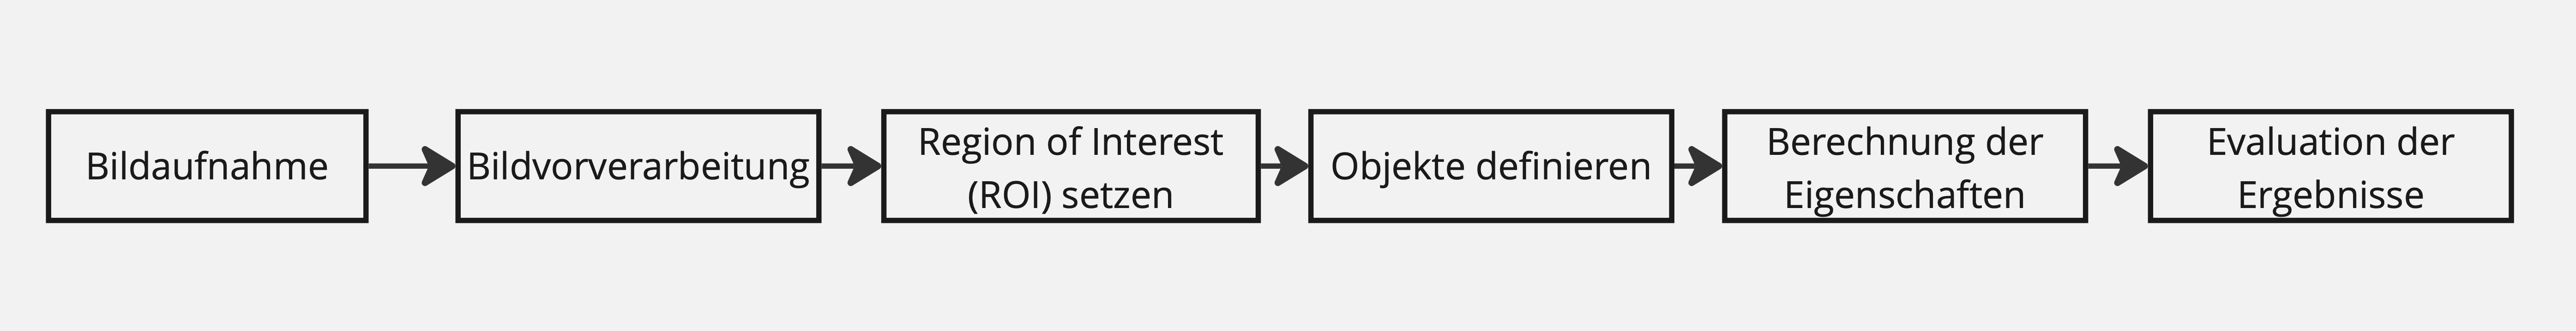
\includegraphics[width=1\linewidth]{expose/Vorgehensmodell_IBV.jpg}
    \caption{Vorgehensmodell der industriellen Sichtprüfung laut \cite[S.15]{demant_industrielle_2011}}
    \label{fig:vorgehensmodell}
\end{figure}

Für eine exakte Objekterkennung ist es in vielen Fällen erforderlich, die genannten Schritte mehrfach zu durchlaufen und \textbf{die Parameter}(besser die Parameter erklären) anzupassen. Dies stellt jedoch lediglich eine einfache Aufgabe dar, sofern sich ein Objekt klar vom Hintergrund unterscheidet. Eigenschaften wie spezielle Texturen, Formen, Farben oder Größen von Objekten können die zuverlässige Detektion erschweren, da Fehler mit dem Hintergrund verschmelzen und somit eine präzise Analyse verhindern. Dies wird durch die Beispiele in Abbildung \ref{fig:image2} verdeutlicht, die Fälle darstellen, die in der Praxis nicht mit traditionellen Algorithmen gelöst werden können.

\begin{figure}[h]

\begin{subfigure}{0.5\textwidth}
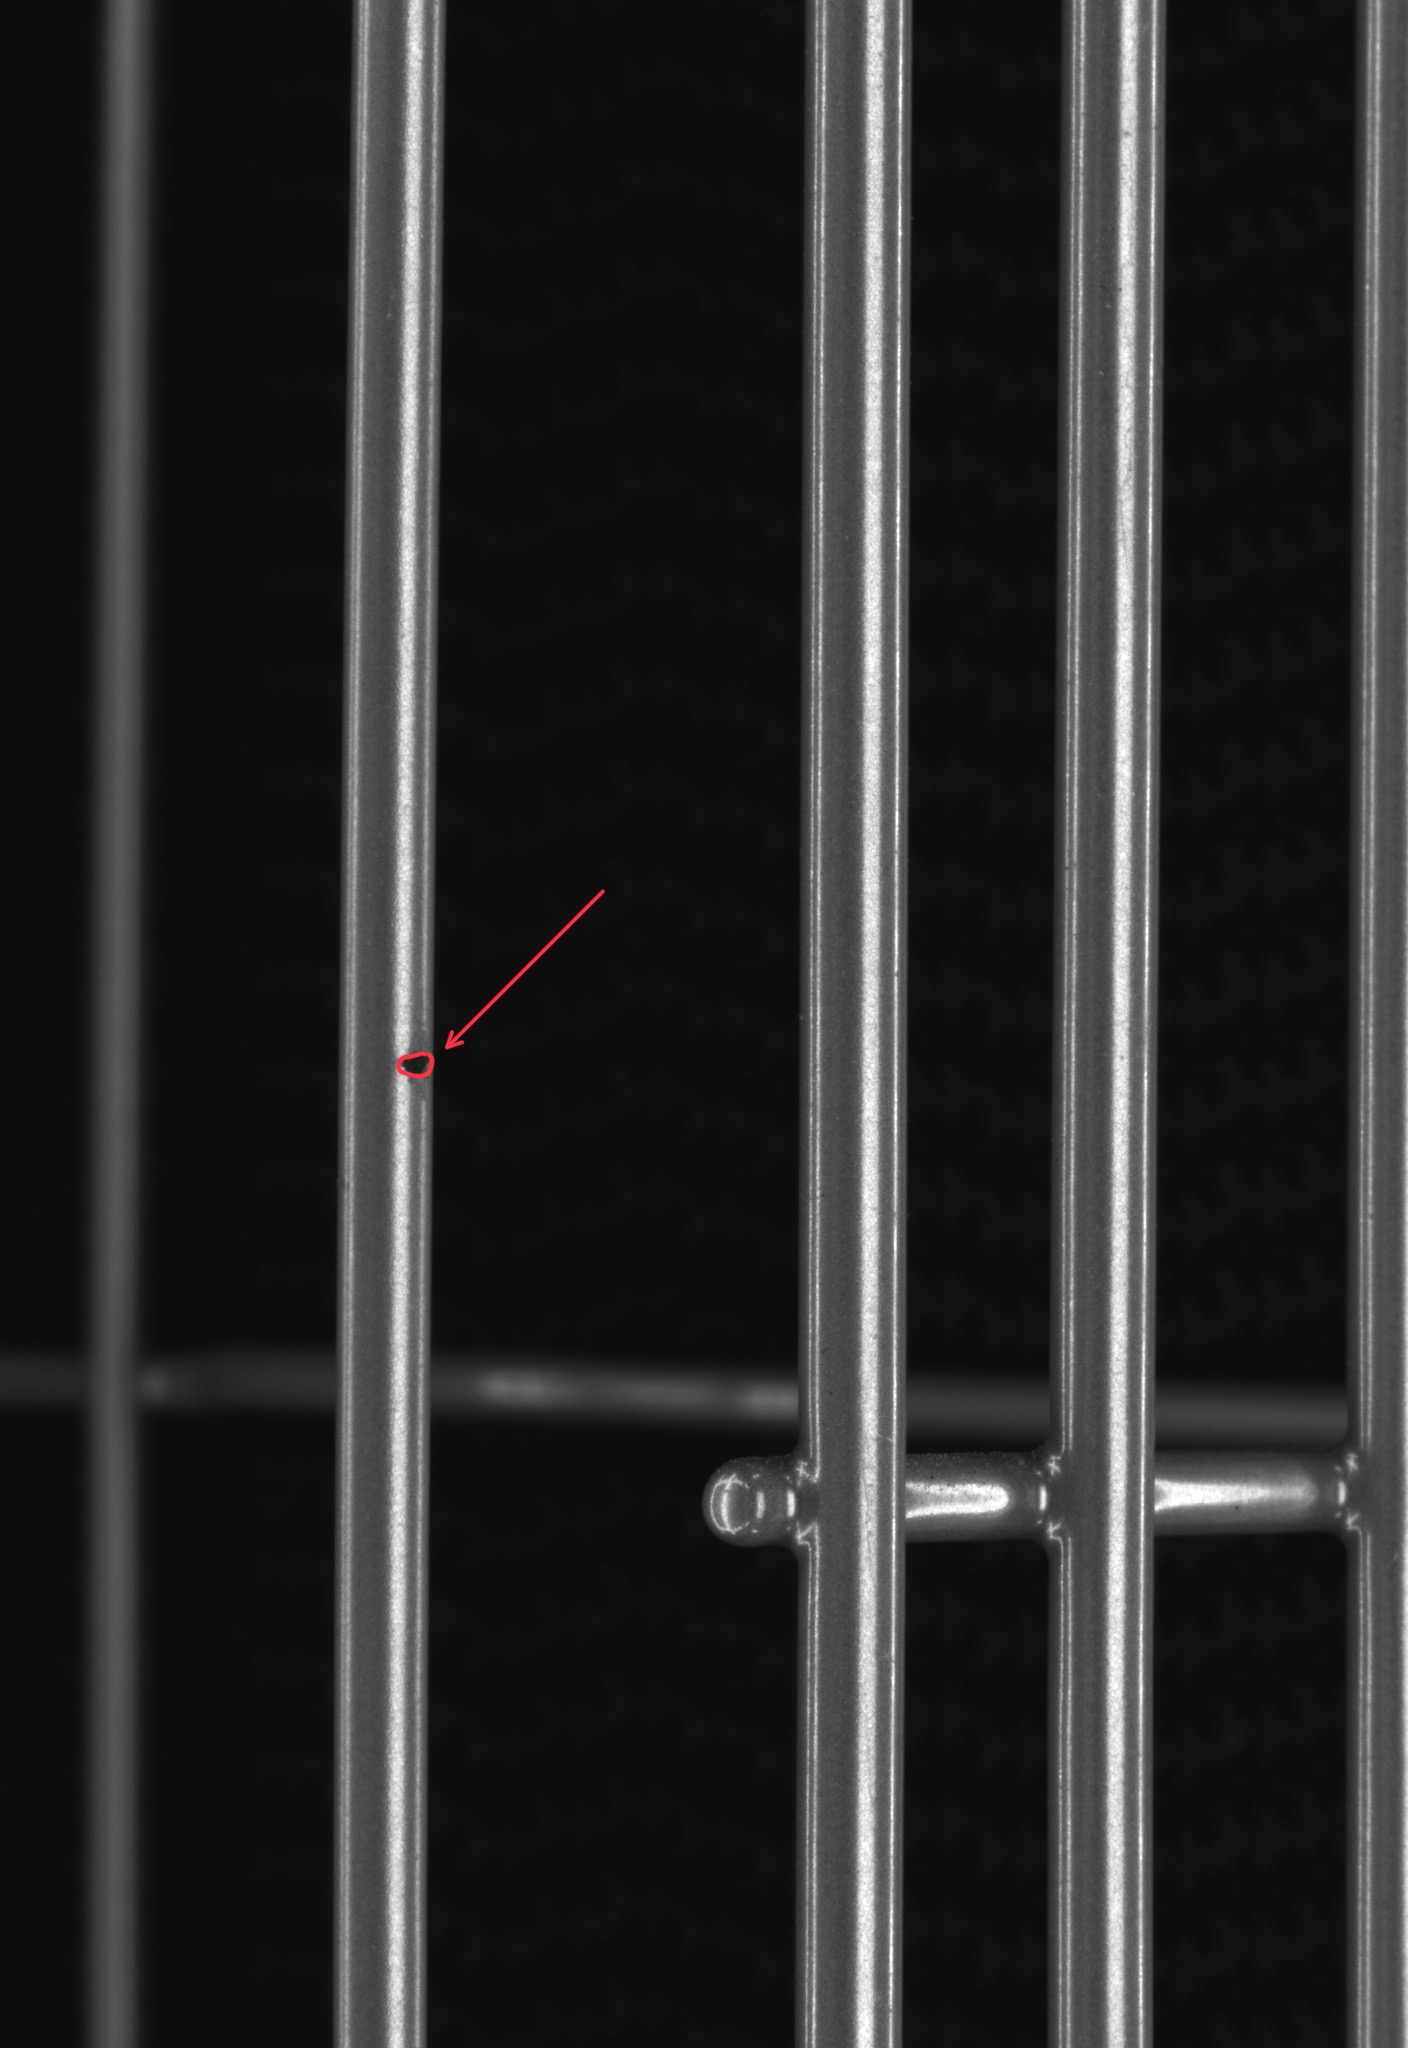
\includegraphics[width=0.9\linewidth, height=6cm]{expose/Fehler.jpg} 
\caption{Verschmutzung an einem Draht; das gesuchte Merkmal ist aufgrund seiner geringen Größe kaum zu erkennen. Die Verschmutzungen haben denselben Grauwert wie der Hintergrund.}
\label{fig:subim1}
\end{subfigure}
\begin{subfigure}{0.5\textwidth}
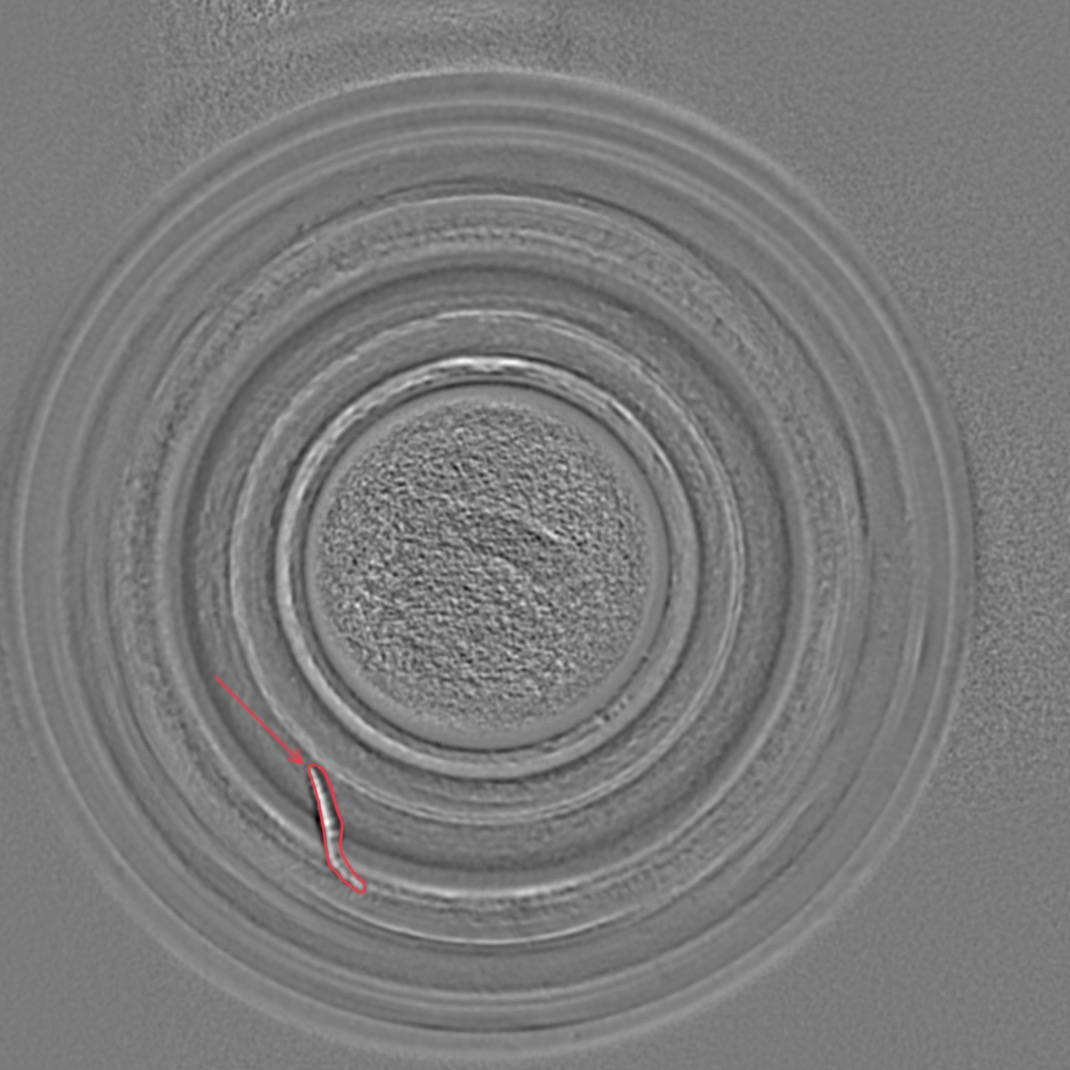
\includegraphics[width=0.9\linewidth, height=6cm]{expose/Kratzer.jpg}
\caption{Kratzer an einem Musterteil; die Fehler weisen sehr ähnliche Muster wie die fehlerfreien Abschnitte des Musterteils auf. Die Graustufen des gesuchten Merkmals ähneln stark denen des Bildhintergrunds.}
\label{fig:subim2}
\end{subfigure}

\caption{Beispiele aus der Praxis der Sichtprüfung. Die Bilder wurden bereits mittels Bildvorverarbeitungsalgorithmen verbessert, um eine höhere Bildqualität zu erzielen. Die gesuchten Merkmale wurden händisch gekennzeichnet, um dem Leser einen Überblick zu verschaffen.}

\label{fig:image2}
\end{figure}

Durch die tiefen Schichten neuronaler Netze können komplexe Merkmalsrepräsentationen gelernt werden, die feinere Details und abstrakte Muster erkennen lassen. Beispielsweise haben \gls{cnn} in der Oberflächeninspektion hohe Genauigkeiten bei der Erkennung von Defekten auf Metalloberflächen erreicht \citep{saberironaghi_defect_2023}.

Angesichts dieser Fortschritte möchte ich in meiner Arbeit untersuchen, wie \gls{dl}-Methoden. Ziel ist es zu demonstrieren, dass mithilfe dieser Methoden auch in anspruchsvollen Szenarien eine präzise Objekterkennung und Segmentierung möglich ist, in denen traditionelle Methoden versagen.

\section{Problemstellung}\label{problemstellung}

Ein Beispiel für den Einsatz von \gls{dl}-Modellen in der \gls{ibv} ist ShuffleDefectNet, das auf dem NEU-Datensatz eine Genauigkeit von 99,75 \% erreichte \cite{saberironaghi_defect_2023}. Dieses Modell erfordert eine große Anzahl von fehlerfreien und fehlerhaften Beispielen in den Trainingsdaten. Es wird mit korrekt gelabelten Daten trainiert, um zwischen fehlerfreien und fehlerhaften Mustern zu unterscheiden. Der NEU-Datensatz umfasst insgesamt 1.800 Bilder, die in sechs verschiedene Defektklassen mit jeweils 300 Bildern unterteilt sind.

Im Gegensatz dazu sind Bildverarbeitungsaufgaben aus der Praxis meist auf spezifische Produkte, Materialien oder Defekte fokussiert. Ein industrieller Datensatz könnte beispielsweise ausschließlich Bilder eines speziellen Musterteils mit bestimmten Arten von Kratzern oder Defekten enthalten. Da es für verschiedene Anwendungsfälle keine öffentlich zugänglichen Datensätze gibt, entstehen häufig relativ kleine Datensätze, deren zu detektierende Merkmale oder Regionen in den Bildern manuell annotiert werden müssen.

Zusammenfassend besteht die Problemstellung darin:

\begin{itemize} 
\item \textbf{Spezialisierte Aufgabenstellung}: Das Modell soll spezifische Merkmale oder Anomalien erkennen, die nur in diesem speziellen Kontext relevant sind. 
\item \textbf{Begrenzte Datenmenge}: Aufgrund der Spezialisierung ist die Anzahl der verfügbaren Trainingsdaten oft gering. Es ist aufwändig und kostspielig, große Mengen an industriellen Bilddaten zu sammeln und zu annotieren, insbesondere wenn es um seltene Defekte oder spezifische Produktionsbedingungen geht. 
\end{itemize}

Künstliche neuronale Netze (\gls{knn}) erfordern in der Regel große Datenmengen, wenn sie mittels überwachtem Lernen trainiert werden, um eine gute Generalisierungsfähigkeit zu entwickeln und somit zuverlässige Ergebnisse zu liefern \cite{lecun_deep_2015}.

Im Rahmen dieser Arbeit sind die Fortschritte im medizinischen Bereich von besonderem Interesse, da die dortigen Herausforderungen denen unseres Datensatzes ähneln. Ein Beispiel dafür ist das U-Net-Modell von Ronneberger et al. (2015) \cite{ronneberger_u-net_2015}, das speziell für die effiziente Segmentierung komplexer Mikroskopiebilder in der Biomedizin entwickelt wurde.

Das U-Net-Modell kann mit sehr wenigen Bildern trainiert werden und zeigt dennoch eine überlegene Leistung bei Aufgaben der biomedizinischen Bildsegmentierung. Es nutzt intensiv Datenaugmentation, um die begrenzte Anzahl annotierter Beispiele effizient zu nutzen.

In den letzten Jahren wurde die U-Net-Architektur erfolgreich in verschiedenen Bereichen der Medizin eingesetzt \cite{azad_medical_2024, siddique_u-net_2021}. Ihre Anpassungsfähigkeit und Effizienz bei der Verarbeitung eingeschränkter Trainingsdaten und stark verrauschter Bilder legen nahe, dass sie auch für die Herausforderungen in der industriellen Bildverarbeitung geeignet sein könnte.

Zwar stehen industrielle Anwendungen im Vordergrund dieser Arbeit; die Methoden werden jedoch allgemein entworfen, um auch auf andere Aufgaben adaptierbar zu sein.

\section{Zielsetzung}\label{zielsetzung}

Das Ziel dieser Bachelorarbeit ist es, die Erkennungsgenauigkeit von Objekten in industriellen Bildern mithilfe eines leicht modifizerten U-Net-Modells zu maximieren. Dabei werden insbesondere Herausforderungen wie starkes Bildrauschen und begrenzte Datenmengen adressiert.
Zur Zielerreichung wird die U-Net-Architektur angepasst und optimiert, indem die spezifischen Eigenschaften der Bilddaten analysiert und die Hyperparameter abgestimmt werden. PyTorch dient als Implementierungs-Framework. Eine umfassende Literaturrecherche wird den aktuellen Stand der Technik im Bereich der \gls{dl}-basierten \gls{oe} beleuchten und aktuelle Trends, Herausforderungen sowie Lösungsansätze identifizieren. Abschließend erfolgt eine systematische Evaluierung der Modellleistung, um die Genauigkeit und Effizienz der Objektdetektion zu bewerten. Dies soll zu optimalen Strategien für die industrielle Qualitätskontrolle beitragen.

\subsubsection{Forschungsfragen}

\begin{enumerate}

\item Wie effektiv kann das U-Net-Modell mittels semantischer Segmentierung gelabelte Merkmale in stark verrauschten industriellen Bildern detektieren, und welche Genauigkeit lässt sich dabei erreichen?

\item Welche Methoden der Datenvorbereitung (z.B. Datenaugmentation, Bildvorverarbeitung) und der Modellanpassung (z.B. Architekturmodifikationen, Hyperparameter Tuning ) können die Leistungsfähigkeit des U-Net-Modells unter den Bedingungen von starkem Bildrauschen und begrenzter Datenmenge verbessern?

\end{enumerate}

    \chapter{Literaturrecherche und Stand der Technik}\label{sec:stand_der_technik}

Es gibt zahlreiche Ratgeber\index{Ratgeber} für das wissenschaftliche Arbeiten und Schreiben. Die Handbücher unterscheiden sich in inhaltlichen Schwerpunkt, praktischer Orientierung und Vertiefung der einzelnen Themen. Drei sehr empfehlenswerte Ratgeber sollen kurz vorgestellt werden.

\cite{karmasin2012gestaltung} bieten einen sehr knappen und praktisch orientierten Ratgeber. Es werden inhaltliche und formale Anforderungen an wissenschaftliche Arbeiten wie inhaltlicher Aufbau der Kapitel, Bewertungskriterien und formale Aspekte wie Gliederung behandelt. Daneben enthält der Ratgeber ein eigenes Kapitel mit Tipps zur Formatierung mit Word.

Das Handbuch von \cite{esselborn2012richtig} konzentriert sich auf die Frage nach dem richtigen wissenschaftlichen Sprachstil. Es werden konkrete Regeln und Übungen vorgestellt um sprachliche Präzision und gedankliche Klarheit im Text zu erreichen. Daneben wird in einem eigenen Kapitel auf die häufigsten Fehler beim wissenschaftlichen Schreiben hingewiesen.

\cite{balzert2011wissenschaftliches} bieten einen sehr ausführlichen Ratgeber zum wissenschaftlichen Arbeiten. Im ersten Teil werden Qualitätskriterien und Methoden als Grundlagen wissenschaftlicher Arbeit aufgezeigt. Im zweiten Teil werden verschiedene wissenschaftliche Artefakte also Textformen gegenübergestellt und der formale Aufbau wissenschaftlicher Arbeiten beleuchtet. Im dritten Teil werden Empfehlungen zum Erstellungsprozess einer Arbeit mit Projektplan etc. gegeben. Im letzten Teil werden verschiedene Aspekte der Präsentation behandelt, wie z. B. Vortragsformen mit und ohne visuelle Unterstützung oder der richtige Vortragsstil.

\section{Überblick über die Industrielle Bildverarbeitung}

\section{Deep Learning in der Bildverarbeitung}

\section{Aktuelle Forschung und Entwicklungen}


    \chapter{Präparierung der Bilddaten}\label{sec:Bilddaten}
[Text]

\section{Beschreibung des Datensatzes}

\section{Labeling-Prozess}

\section{Datenaugumentationstechniken}


    \chapter{Implementierung und Experimente}\label{sec:model_implement}

\section{Präparierung der Bilddaten}
\subsection{Vorbereitung und Beschreibung des Datensatzes}
\subsection{Labeling-Prozess}
\subsection{Datenaugmentationstechniken}

\section{Modellierung und Training}
\subsection{Auswahl der Softwarebibliotheken} 
\subsection{Modellarchitektur}
\subsection{Trainingsprozess und Hyperparameter-Optimierung}
\section{Validierung und Bewertung der Ergebnisse}
\subsection{Methoden der Validierung}
\subsection{Bewertungsmethoden und Metriken}
\subsection{Analyse und Diskussion der Ergebnisse}

   % \chapter{Validierung und Bewertng der Ergebnisse}\label{sec:validierung}
[Text]

\section{Methoden der Validierung}

\section{Bewertungsmethoden und Metriken}

\section{Analyse und Diskussion der Ergebnisse}

    \chapter{Fazit und Ausblick}\label{sec:Fazit}

Die hier vorliegende Dokumentvorlage soll die Gestaltung wissenschaftlicher Arbeiten am Lehrstuhl für Medieninformatik erleichtern und zur Qualitätssicherung beitragen. Es werden Richtlinien für den inhaltlichen Aufbau und die formale Gestaltung formuliert. Dabei ist die Vorlage selbst wie eine wissenschaftliche Arbeit strukturiert und enthält die wichtigsten Formatvorlagen zur effizienten Gestaltung mit Word. Als zusätzliches Hilfsmittel für den inhaltlichen Aufbau verschiedener Arbeiten befinden sich im Anhang typische Bausteine bzw. Mustergliederungen für verschiedene Thementypen, wie „theoretische“, „konstruktive“ oder „empirische“ Arbeiten. Für weitere Informationen sind im Kapitel \ref{sec:stand_der_technik} verschiedene Ratgeber kurz vorgestellt. 

\section{Zusammenfassung der Ergebnisse}

\section{Diskussion der Ergebnisse}

\section{Ausblick auf Zukünftige Arbeiten}

    
    % Kapitelbezeichnung in der rechten oberen Ecke entfernen
\clearpage
\pagestyle{plain}
    
% Literaturverzeichnis anzeigen
% kleinerer Zeilenabstand, damit es nicht so gestreckt aussieht
\onehalfspacing
\bibliography{references}
\doublespacing

\end{document}
